% Options for packages loaded elsewhere
\PassOptionsToPackage{unicode}{hyperref}
\PassOptionsToPackage{hyphens}{url}
%
\documentclass[
]{article}
\title{R Markdown Lesson 03: Keeping Calm}
\author{Alexander Strobel \& Christoph Scheffel}
\date{}

\usepackage{amsmath,amssymb}
\usepackage{lmodern}
\usepackage{iftex}
\ifPDFTeX
  \usepackage[T1]{fontenc}
  \usepackage[utf8]{inputenc}
  \usepackage{textcomp} % provide euro and other symbols
\else % if luatex or xetex
  \usepackage{unicode-math}
  \defaultfontfeatures{Scale=MatchLowercase}
  \defaultfontfeatures[\rmfamily]{Ligatures=TeX,Scale=1}
\fi
% Use upquote if available, for straight quotes in verbatim environments
\IfFileExists{upquote.sty}{\usepackage{upquote}}{}
\IfFileExists{microtype.sty}{% use microtype if available
  \usepackage[]{microtype}
  \UseMicrotypeSet[protrusion]{basicmath} % disable protrusion for tt fonts
}{}
\makeatletter
\@ifundefined{KOMAClassName}{% if non-KOMA class
  \IfFileExists{parskip.sty}{%
    \usepackage{parskip}
  }{% else
    \setlength{\parindent}{0pt}
    \setlength{\parskip}{6pt plus 2pt minus 1pt}}
}{% if KOMA class
  \KOMAoptions{parskip=half}}
\makeatother
\usepackage{xcolor}
\IfFileExists{xurl.sty}{\usepackage{xurl}}{} % add URL line breaks if available
\IfFileExists{bookmark.sty}{\usepackage{bookmark}}{\usepackage{hyperref}}
\hypersetup{
  pdftitle={R Markdown Lesson 03: Keeping Calm},
  pdfauthor={Alexander Strobel \& Christoph Scheffel},
  hidelinks,
  pdfcreator={LaTeX via pandoc}}
\urlstyle{same} % disable monospaced font for URLs
\usepackage[margin=1in]{geometry}
\usepackage{graphicx}
\makeatletter
\def\maxwidth{\ifdim\Gin@nat@width>\linewidth\linewidth\else\Gin@nat@width\fi}
\def\maxheight{\ifdim\Gin@nat@height>\textheight\textheight\else\Gin@nat@height\fi}
\makeatother
% Scale images if necessary, so that they will not overflow the page
% margins by default, and it is still possible to overwrite the defaults
% using explicit options in \includegraphics[width, height, ...]{}
\setkeys{Gin}{width=\maxwidth,height=\maxheight,keepaspectratio}
% Set default figure placement to htbp
\makeatletter
\def\fps@figure{htbp}
\makeatother
\setlength{\emergencystretch}{3em} % prevent overfull lines
\providecommand{\tightlist}{%
  \setlength{\itemsep}{0pt}\setlength{\parskip}{0pt}}
\setcounter{secnumdepth}{-\maxdimen} % remove section numbering
\newlength{\cslhangindent}
\setlength{\cslhangindent}{1.5em}
\newlength{\csllabelwidth}
\setlength{\csllabelwidth}{3em}
\newlength{\cslentryspacingunit} % times entry-spacing
\setlength{\cslentryspacingunit}{\parskip}
\newenvironment{CSLReferences}[2] % #1 hanging-ident, #2 entry spacing
 {% don't indent paragraphs
  \setlength{\parindent}{0pt}
  % turn on hanging indent if param 1 is 1
  \ifodd #1
  \let\oldpar\par
  \def\par{\hangindent=\cslhangindent\oldpar}
  \fi
  % set entry spacing
  \setlength{\parskip}{#2\cslentryspacingunit}
 }%
 {}
\usepackage{calc}
\newcommand{\CSLBlock}[1]{#1\hfill\break}
\newcommand{\CSLLeftMargin}[1]{\parbox[t]{\csllabelwidth}{#1}}
\newcommand{\CSLRightInline}[1]{\parbox[t]{\linewidth - \csllabelwidth}{#1}\break}
\newcommand{\CSLIndent}[1]{\hspace{\cslhangindent}#1}
\ifLuaTeX
  \usepackage{selnolig}  % disable illegal ligatures
\fi

\begin{document}
\maketitle

\hypertarget{outline}{%
\section{Outline}\label{outline}}

In this lesson, we elaborate on the last one, especially on how to

\begin{itemize}
\tightlist
\item
  use a BibTeX library as reference manager
\item
  write custom code for your analysis pipeline without resorting to real
  data
\item
  format tables and figures as well as their legends
\end{itemize}

\hypertarget{use-a-bibtex-library-as-reference-manager}{%
\section{Use a BibTeX library as reference
manager}\label{use-a-bibtex-library-as-reference-manager}}

As you alredy learned, RMarkdown uses LaTeX for formatting. Usually,
LaTeX uses BibTex as citation format (but apparently, you can also use
\href{https://citeproc-js.readthedocs.io/en/latest/csl-json/markup.html}{CSL-JSON},
if you are familiar with that option). To ensure that everything works
properly, make sure that you stated the name of the BibTeX file (via
bibilography:) as well as the Citation Style Language (via csl:) in the
YAML header (see top of the R Markdown document).

You can fetch BibTeX formatted references from the web using, e.g.,
JabRef (\url{https://www.jabref.org/}) or import them from Endnote via
the BibTeX Export output style that can be downloaded from the Endnote
web site und the following URL:
\url{https://endnote.com/style_download/bibtex-export/} Double-click it,
which should load it into Endnote, and then (under Edit) set it as
Output Citation Style. Then export your Endnote file via
File\textgreater Export to the desired location (please note that if you
want to keep the old name and save the BibTex file to the same folder as
the original file this might not work. Therefore, choose another
filename or folder). For other citation managers, there are surely also
options to get BibTex formatted entries. For Zotero, \emph{papaja} (more
on this package in the next lesson) offers a special function called
fetch\_zotero\_refs that we have not tried yet.

You can then simply paste the BibTeX entries into your BibTeX file, but
make yourself familiar with the BibTeX format to avoid frustration (see
here: \url{https://www.openoffice.org/bibliographic/bibtex-defs.html}).
Here is an examplary BibTeX entry:

\begin{quote}
\begin{tabbing}
@Article\{Gignac2016,\\
\hspace{1em} \= author = \{G. E. Gignac  and E. T. Szodorai\},\\
\hspace{1em} \= title = \{Effect size guidelines for individual differences researchers\},\\
\hspace{1em} \= journal = \{Personality and Individual Differences\},\\
\hspace{1em} \= year = \{2016\},\\
\hspace{1em} \= volume = \{102\},\\
\hspace{1em} \= pages = \{74-78\},\\
\hspace{1em} \= doi = \{10.1016/j.paid.2016.06.069\},\\
\}
\end{tabbing}
\end{quote}

One important usage hint is that BibTex sets all letters of the title
except the first to lowercase, which is not a bug, but a feature, as
that way, automatically imported titles that happen to comprise
uppercase words are correctly printed as lowercase. Likewise, all first
letters of journal names are printed uppercase. If you want to retain
uppercase or lowercase, put the respective letter in \{\}. Another issue
is how to handle special characters such as ä, á, ê, ñ or ß. You can do
this via \{\textbackslash``a\} \{\textbackslash´a\}
\{\textbackslash\^{}e\} \{\textbackslash\textasciitilde n\} or
\{\textbackslash ss\}.

In order to reduce a lot of editing, I wrote a function called
\emph{editbib} (see resources folder). Source the \emph{editbib}
function in R and then simply type

\begin{quote}
editbib(infile=[path/name of exported Endnote file], outfile=[path/name of new file])
\end{quote}

\emph{editbib} will then rename all references labels to AuthorYear
(e.g., Strobel2018), will remove possible spaces in author names
(e.g.~in von Stumm) and handle some of the more common special
characters. If you want to replace further characters, find out their
so-called escape sequence. A comprehensive list of escape sequences can
be found at:
\url{https://www.rpi.edu/dept/arc/training/latex/LaTeX_symbols.pdf}. Via
the arguments \emph{add.special} and \emph{add.replace}, you can then
tell \emph{editbib} the additional characters to handle.

Yes, we know this is a lot of work, it's so much easier with Word and
Endnote, and indeed, it is! Yet, doing good and open science is hard and
often frustrating work. However, all the work you invested initially
will payout in the end because you will regain control of your work. And
keep in mind, other people have already solved most of the hard stuff.
And once you have set up your BibTeX library, citing is quite
straightforward: To cite some reference, just write something like ``For
the present work, we used recently established effect size guidelines
for correlations (Gignac \& Szodorai, 2016).'' to have the reference
cited in parentheses or ``For the present work, we used the effect size
guidelines for correlations recently established by Gignac \& Szodorai
(2016).''

\hypertarget{write-custom-code-for-your-analysis-pipeline}{%
\section{Write custom code for your analysis
pipeline}\label{write-custom-code-for-your-analysis-pipeline}}

\hypertarget{the-problem}{%
\subsection{The problem}\label{the-problem}}

In the last lessons, we have introduced several functions that evaluate
the outcome of some statistical analysis (such as effect size
magnitudes) or report the results in a prespecified way (such as
correlations with 95\% confidence intervals and \(p\)-values). Given
that you want to write an analysis pipeline for, say, a registered
report, this is especially important, because you can deliver the
analysis code for testing your preregistered hypotheses already along
with your registered report, which certainly enhances your chances in
the Stage 1 review process. Yet, usually, you do not yet have data to
test your analysis pipeline. One way would be to collect some pilot
data, but the sample size would probably be too small to allow for
certain decisions to be made along the way. Another way would,
therefore, be to simulate data, add some noise, and check your routines
with these simulated data.

In the following, we will follow the latter path by assuming that we
want to run some really boring analysis: We will have three
cross-sectionally measured self-report variables that we want to include
in a mediation model (the pros and cons of such an analysis plan put
aside for now). The the `independent' variable \(X\), the `dependent'
variable \(Y\), and the mediator variable \(Z\) are measured as
continuous measures, but we cannot be sure whether they are normally
distributed. Therefore, (univariate or multivariate) normality tests
will have to be performed, decisions on data normalization,
transformation, and outlier exclusions will have to be considered and
ideally predetermined -- and all in your pre-written code! That is, you
have to be (and ultimately \emph{will} be) prepared to eventually load
the real data into your R Markdown script, execute your prespecified
analysis at a glance and produce the results section of your manuscript
in no longer than a few seconds (or minutes, depending on the complexity
of your analyses).

\hypertarget{the-garden-of-forking-paths}{%
\subsection{The garden of forking
paths}\label{the-garden-of-forking-paths}}

It is wise to take some time in advance and to elaborate on the decision
tree (AKA the \emph{garden of forking paths}) that you can imagine.
Let's say you first consider to check for missing values in your data.
Even at this stage, you have the choice to (1) remove cases with missing
values or (2) impute missing values. Choice option (1) would be
advisable if there are a lot of missing values in the self-report
measures of some participants, while with only a couple of missings,
choice option (2), i.e., imputation, might seem prefereable. But what,
if you have both: Several participants skipped a whole page of some
questionnaire, while others filled in most, but not all items of the
questionnaires. This would most probably result in a two-step approach:
firstly, remove all participants who have more than some prespecified
number of missings (but how much is tolerable?), and secondly, impute
missings for the remainder of the participants (but by using which
imputation method?).

Also, exclusion of outliers might be challenging: Do you remove
univariate outliers by means of boxplots where outliers are defined as
values 1.5 interquartile ranges (IQR) above or below the box? Or aren't
the outliers rather the extreme values beyond 3 IQR? And what, if after
removel of the outliers via boxplots, a new boxplot reeals new outliers?
Or do you rather remove outliers by means of multivariate analyses such
as Mahalanobis distances? And if so, what is your criterion for doing
so?

To complicate matters even further: If you choose univariate normality
tests, do you opt for normalizing variables (i.e., trying to make them
more `normal' by ranking the data and then transforming the rank order
to the normal distribution)? And if you opt for normalizing, what would
be the algorithm used to do so (there are at least four of them)? And do
you normalize ahead of removing outliers or afterwards?

And finally: do you -- depending on the final data (quality) or per
default -- use standard/parametric or nonparametric/robust tests such as
Pearson correlations and linear regression or rather Spearman
correlations and robust regression (and if so, using which algorithm)?
May you rather consider the estimation of Bayes factors and posterior
estimates for your correlation/regression coefficients instead of
standard frequentist analyses? And if so, is there a sound approach to
Bayesian mediation analysis? Certainly, there are multiple, seemingly
sound approaches, but which one to choose?

This simple example -- three variables to correlate and then to put into
a mediation model, which does not seem to be too hard a problem, might
well illustrate the vast amount of degrees of freedom you have in
statistical analyses. Still, we have to keep calm and carry on! In an
ideal world, we would sketch all the forking paths and discuss them with
our peers, which more likely than not would result in a high degree of
disagreement and additional forking paths, so voting on the to be
preferred path might be an option to set up our analysis pipeline. Even
better, we would run all other (or at least all other -- judging from
our peers' votes -- \emph{plausible}) paths and add the respective
results to a supplement of our forthcoming paper.

\hypertarget{the-present-approach}{%
\subsection{The present approach}\label{the-present-approach}}

Yet, it would go beyond the scope of this R Markdown course if we would
elaborate on the decisions to be made during the specification of our
analysis plan. For this lesson, we will assume data and analysis steps
as follows:

\begin{itemize}
\tightlist
\item
  we have no missings in the data, but \(N=256\) observations\footnote{Why
    do we have \(N=256\) participants? Firstly, 256 is a power of 2
    which is always a good number. Yet, secondly and more importantly,
    if you do correlation analysis, you need to make sure to arrive at
    stable estimates, which in simulations by Schönbrodt \& Perugini
    (2013) usually is the case only if your sample size is N \(\ge\)
    250.} of the variables \(X\), \(Y\), and \(Z\), with internal
  consistencies of \(\alpha_{X}=.82\), \(\alpha_{Y}=.76\), and
  \(\alpha_{Z}=.79\)
\item
  the data are somewhat skewed and do not fully conform to either
  univariate or multivariate normality
\item
  there are some outliers, the exclusion of which on the basis of a test
  for multivariate normality ameliorates data quality
\item
  depending on whether there is still deviation from normality, we use
  either Pearson correlations and standard linear Regression or robust
  variants, i.e., Spearman correlations and robust regression
\item
  for testing the indirect effect in our mediation model, we use
  bootstrapping and extract bias-corrected and accelerated confidence
  intervals
\end{itemize}

In what follows, routines are established that report and evaluate the
results of our analyses without knowing in advance what they look like.

\hypertarget{the-analysis-pipeline}{%
\subsection{The analysis pipeline}\label{the-analysis-pipeline}}

We first simulate three correlated variables \(X\), \(Y\), and \(Z\)
from a normal distribution with \(\mu=0\) and \(\sigma=1\). We then add
some noise by randomly assigning four data points in \(Y\) and \(Z\)
with values from a uniform distribution with \(min=3.75\) and
\(max=4.25\). We then retrieve descriptives including skew and kurtosis,
run a Shapiro-Wilk test for univariate normality and a Mardia test for
multivariate normality and identify possible multivariate outliers based
on squared Mahalanobis distances. After reporting and illustrating the
descriptive results., we run the actual statistical tests. Depending on
the distribution characteristics observed, we either run standard
correlation and regression analyses, i.e., Pearson correlation and
standard linear regression, or robust alternatives, i.e.~Spearman
correlations and robust regression. We also state which versions of R
and RStudio we used and which packages we employed. This is not only
done to give proper credit, but also because for some statistical
procedures, it can make a difference which version of R and/or R
packages one was using when it comes to reproduce the results.
Therefore, we state that we used R (R Core Team, 2018) with RStudio
(RStudio Team, 2016) and employed the package \emph{psych} (Revelle,
2018).

\begin{figure}[bt]

{\centering 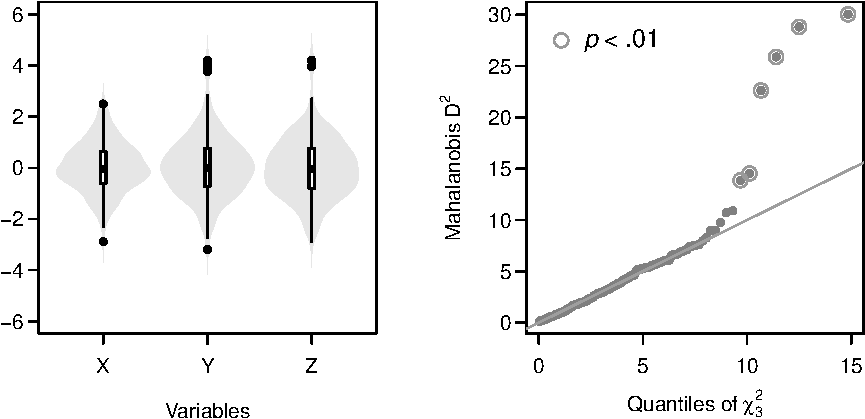
\includegraphics{RM_03_KeepingCalm_files/figure-latex/analysis.1-1} 

}

\caption{Distributions of the examined variables. The left panel gives boxplots, the right panel gives QQ-plots of the squared Mahalanobis distances, plottet against the theoretical quantiles.}\label{fig:analysis.1}
\end{figure}

\hypertarget{customize-the-reporting-of-results-in-the-body-of-the-manuscript}{%
\subsection{Customize the reporting of results in the body of the
manuscript}\label{customize-the-reporting-of-results-in-the-body-of-the-manuscript}}

Here is an example text for a Results section: ``Shapiro-Wilk tests for
deviation from univariate normality showed that variable \(X\) did not
deviate from the normal distribution, \(p>.2\), while variables \(Y\)
and \(Z\) deviated from the normal distribution, \(p<.2\), see Table 1
for details. Furthermore, a Mardia test for multivariate normality
indicated that there was a deviation from the multivariate normal
distribution, \(p_{skew}\) \textless{} .001, \(p_{kurtosis}\)
\textless{} .001. The left panel of Figure 1 gives the distribution of
the examined variables including boxplots and possible univariate
outliers, i.e., values above or below 1.5 interquartile ranges from the
borders of the box. The right panel of Figure 1 gives the squared
Mahalanobis distances per participant, plotted against the theoretical
quantiles of the \(\chi^2\) distribution with \(df=3\). Multivariate
outliers, i.e., Mahalanobis distances that under a \(\chi^2\)
distribution with \(df=3\) have a probability of \(p<.01\) are marked.
Given the overall non-normal distribution of the data, we computed
Spearman correlations and robust regression to test our hypotheses.''

As you can see in the R Markdown source document, there are a number of
placeholders in the text. Take a look at the source text for the first
sentence of the Results and also at the R code chunk ahead of this
paragraph (see under the comment \# add results from shapiro.tests).
Here, deviation from univariate normality is first determined, and then
depending on which and how many variables deviate from the normal
distribution, the text elements to insert in the Results section are
defined. If only one variable is non-normally distributed, the text
element \emph{variable} will appear; if there are two non-normally
distributed variables, the text element will appear as \emph{variables}.
That means that you carefully have to consider what would be possible
outcomes of different analysis steps that would affect your decision
tree in what way and to generate text elements that reflect the nature
of the outcomes as well as what follows from these outcomes with regard
to your decision tree. In the present case, we considered that for the
univariate case, there could be one or two normally or non-normally
distributed variables (but in fact, the code above does not account for
the possibility that all three variables were normally or non-normally
distributed). We also considered that there could be a deviation or no
deviation from multivariate normality. We finally define at the end of
the code chunk how we proceed if there are univariate and/or
multivariate deviations from normality. In our case,
non-parametric/robust tests are performed if there is \emph{any}
deviation, be it univariate or multivariate, but there are certainly
reasons to make a different decision. Still, your decisions how to
analyze your data are fixed in advance, and whatever the results look
like, you are prepared and do not have to edit the reporting part of
your manuscript, not even, when some reviewer requires that you delete
the outliers. In this case, the report would dynamically change, and you
would not have to edit all the tables by hand (which is always
error-prone).

\hypertarget{format-tables-and-figures-as-well-as-their-legends}{%
\section{Format tables and figures as well as their
legends}\label{format-tables-and-figures-as-well-as-their-legends}}

We use the results of the descriptive statistics also to illustrate the
next topic of this lesson: formatting tables and figures. Figure 1 above
already gives an example, and some of its properties such as its height,
alignment, and caption are set in header of the respective code chunk.
In this case, \(fig.height=3.25\) states the height of the figure in
inches, \(fig.pos='bt'\) will make LaTeX try to place the figure first
at the bottom of a page, and if this seems not manageable, then to place
it at the top of the page. Further options would be \('h'\) for placing
the figure approximately at the location in the document where it occurs
in the R Markdown document or \('p'\) for placing the figure on a new
page. Other features are set during the plotting process itself. Please
note that figures that look good when plotted in \emph{RStudio} may
appear a bit bulky in the PDF output, so it may be a good idea to use
values smaller than one for \(cex.axis\) and \(cex.lab\) (these are set
to 0.8 in Figure 1). Also, you might want to consider the placement of
the axes' elements via \(mgp = c(2, .5, 0)\) in Figure 1 (default is
\(mgp = c(3, 1, 0)\) for axis label, tick labels and tick position).
Also, the tick length is adjusted to \(tck = -.03\).

As for tables, the whole thing becomes a bit more tricky, as LaTeX is
not known for its ease in generating tables. Still, in the context of
dynamic, updatable documents, it is worthwhile to consider using R
Markdown instead of Word, because -- as repeatedly underscored -- you
neither will nor want to edit your manuscript by hand when you (may be
forced to) modify your analysis pipeline. In this lesson, we will
provide you with examples for very basic tables only, more complicated,
but also more convenient table options will follow in subsequent
lessons.

\begin{table}[b!]
\begin{center}
\caption{Spearman correlations of the variables of interest}
\vspace{0.25cm}

\begin{tabular}{ l c c c }
  \hline
   & X & Y & Z \\ 
  \hline
   X & \textit{.82} & .13 & .14 \\
   Y & .13 & \textit{.76} & .14 \\
   Z & .14 & .14 & \textit{.79} \\
  \hline  
\end{tabular}
\vspace{0.25cm}

\textit{Note.} $N=$ 256. Coefficients in the diagonal are Cronbach's $\alpha$.
\end{center}
\end{table}

In LaTeX, tables are usually generated like this (code in this knitted
document invisible) and appear like the table below. Let us walk through
the code: First a table environment is generated, and `{[}b!{]}' forces
LaTeX to position the table at the bottom of the page. Then the table is
centered, labeled for cross-referencing and given a caption (that states
whether the correlations are Pearson or Spearman correlations, depending
on the distribution of the variables of interest, see above and R code
chunk \emph{analysis.1}). Then, the actual table is generated with R
chunks embedded that refer to previously computed coefficients to be
provided in the table. A note to the table is inserted at the end.

\begin{figure}
\centering
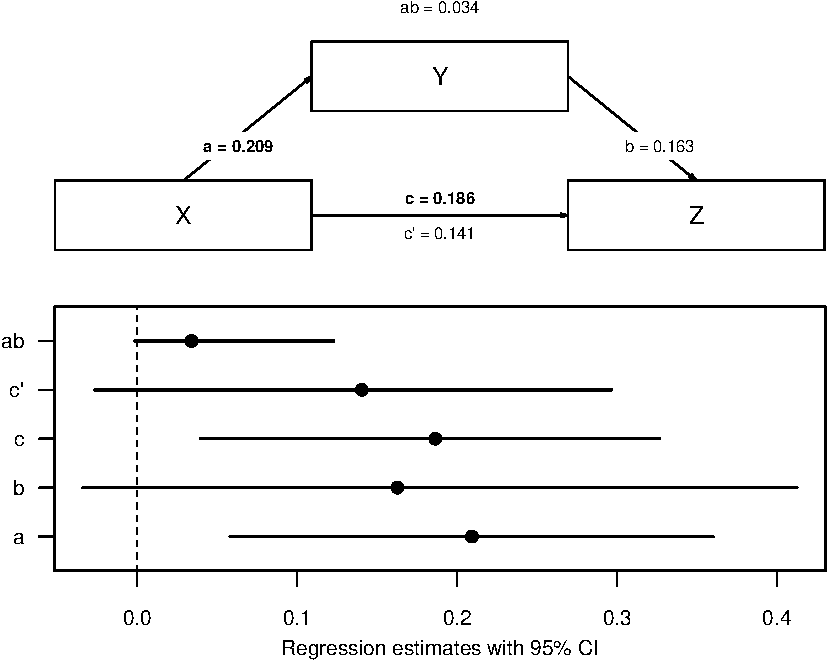
\includegraphics{RM_03_KeepingCalm_files/figure-latex/analysis.3-1.pdf}
\caption{Results of the mediation analysis using robust regression.
Unstandardized coefficients are given and printed bold-faced if their
95\% CI (based on bias-corrected and accelerated bootstrapping with 1000
permutations) does not inlcude zero.}
\end{figure}

Figure 2 gives the results of the mediation analyses. Because no figure
position was defined in the code chunk, it was printed where the figure
best fitted given the position of the R code chunk (you may want to play
around to have the figure positioned on top or the bottom of this page).
We could now go on and provide the results of the mediation analysis in
the main text such as: ``The indirect path was not significant, \(b=\)
0.034, 95\% CI {[}-0.001, 0.123{]}.'' Yet, we will skip any further
reporting of results because we think that the main message is clear
with this example.

\hypertarget{interim-summary}{%
\section{Interim Summary}\label{interim-summary}}

In this lesson, you should have learned how to

\begin{itemize}
\tightlist
\item
  use a BibTeX library as reference manager
\item
  write custom code for your analysis pipeline without resorting to real
  data
\item
  format tables and figures as well as their legends
\end{itemize}

\hypertarget{exercises}{%
\section{Exercises}\label{exercises}}

To exercise what you have learnt in this lesson, you might want to try
the following:

\begin{enumerate}
\def\labelenumi{\arabic{enumi}.}
\tightlist
\item
  Inspect the BibTeX file associated with this document (lesson03.bib)
  to familiarize yourself with the format. Then write new entries for
  the following two references and cite them in the text:

  \begin{itemize}
  \tightlist
  \item
    Cohen, J. (1988). \emph{Statistical power analysis for the
    behavioral sciences.} Hillsdale: Erlbaum.
  \item
    Hemphill, J. F. (2003). Interpreting the magnitudes of correlation
    coefficients. \emph{American Psychologist, 58}(1), 78--80.
  \end{itemize}
\item
  Slightly modify the analysis routine for the correlation analysis to
  compare the results of the appropriate correlation method defined in
  the analysis script with the alternative method, i.e., Spearman
  vs.~Pearson correlations. Provide a table positioned exactly at the
  top of the page with the results of one method above the diagonal and
  the results of the alternative method below the diagonal (and the
  alphas in the diagonal).\\
\item
  Provide a figure with the 95\% confidence intervals of the
  correlations you obtained, for both Spearman and Pearson correlations.
  Depending on which method is indicated by the tests of normality,
  Spearman correlations should be printed in black and Pearson
  correlations in grey (or vice versa). Position the figure exactly at
  the bottom of the page (and don't forget to give it a caption).
\end{enumerate}

\hypertarget{outlook}{%
\section{Outlook}\label{outlook}}

In the next lesson, we will now come to a really helpful R package:
\emph{papaja} that enables you to

\begin{itemize}
\tightlist
\item
  format your R Markdown document
\item
  easily report results of common statistical procedures
\item
  format and place tables and figures
\end{itemize}

all according to APA (albeit 6th edition) style.

\hypertarget{references}{%
\section*{References}\label{references}}
\addcontentsline{toc}{section}{References}

\hypertarget{refs}{}
\begin{CSLReferences}{1}{0}
\leavevmode\vadjust pre{\hypertarget{ref-Gignac2016}{}}%
Gignac, G. E., \& Szodorai, E. T. (2016). Effect size guidelines for
individual differences researchers. \emph{Personality and Individual
Differences}, \emph{102}, 74--78.
\url{https://doi.org/10.1016/j.paid.2016.06.069}

\leavevmode\vadjust pre{\hypertarget{ref-R-base}{}}%
R Core Team. (2018). \emph{R: A language and environment for statistical
computing}. R Foundation for Statistical Computing.
\url{https://www.R-project.org/}

\leavevmode\vadjust pre{\hypertarget{ref-R-psych}{}}%
Revelle, W. (2018). \emph{Psych: Procedures for psychological,
psychometric, and personality research}. Northwestern University.
\url{https://CRAN.R-project.org/package=psych}

\leavevmode\vadjust pre{\hypertarget{ref-RStudio}{}}%
RStudio Team. (2016). \emph{RStudio: Integrated development environment
for {R}}. RStudio, Inc. \url{http://www.rstudio.com/}

\leavevmode\vadjust pre{\hypertarget{ref-Schoenbrodt2013}{}}%
Schönbrodt, F. D., \& Perugini, M. (2013). At what sample size do
correlations stabilize? \emph{Journal of Research in Personality},
\emph{47}, 609--612. \url{https://doi.org/10.1016/j.jrp.2013.05.009}

\end{CSLReferences}

\end{document}
